\documentclass[border=4pt]{standalone}

\usepackage{amsmath}
\usepackage{tikz}
\usepackage{mathdots}
\usepackage{yhmath}
\usepackage{cancel}
\usepackage{color}
\usepackage{siunitx}
\usepackage{array}
\usepackage{multirow}
\usepackage{amssymb}
\usepackage{gensymb}
\usepackage{tabularx}
\usepackage{booktabs}
\usetikzlibrary{fadings}
\usetikzlibrary{patterns}


\begin{document}
 


\tikzset{every picture/.style={line width=0.75pt}} %set default line width to 0.75pt        

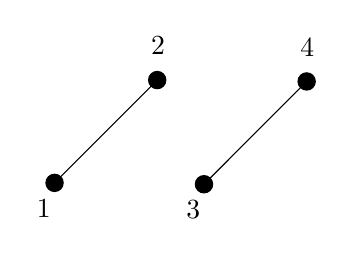
\begin{tikzpicture}[x=0.75pt,y=0.75pt,yscale=-1,xscale=1]
%uncomment if require: \path (0,300); %set diagram left start at 0, and has height of 300

%Shape: Circle [id:dp010300638344936441] 
\draw  [fill={rgb, 255:red, 0; green, 0; blue, 0 }  ,fill opacity=1 ] (81.34,159.7) .. controls (81.34,157.4) and (83.2,155.53) .. (85.5,155.53) .. controls (87.8,155.53) and (89.67,157.4) .. (89.67,159.7) .. controls (89.67,162) and (87.8,163.87) .. (85.5,163.87) .. controls (83.2,163.87) and (81.34,162) .. (81.34,159.7) -- cycle ;
%Shape: Circle [id:dp16687809137287024] 
\draw  [fill={rgb, 255:red, 0; green, 0; blue, 0 }  ,fill opacity=1 ] (130.8,110.17) .. controls (130.8,107.87) and (132.66,106) .. (134.97,106) .. controls (137.27,106) and (139.13,107.87) .. (139.13,110.17) .. controls (139.13,112.47) and (137.27,114.34) .. (134.97,114.34) .. controls (132.66,114.34) and (130.8,112.47) .. (130.8,110.17) -- cycle ;
%Straight Lines [id:da019730710183089473] 
\draw    (134.97,110.17) -- (85.5,159.7) ;


%Shape: Circle [id:dp0875552439686309] 
\draw  [fill={rgb, 255:red, 0; green, 0; blue, 0 }  ,fill opacity=1 ] (153.34,160.37) .. controls (153.34,158.07) and (155.2,156.2) .. (157.5,156.2) .. controls (159.8,156.2) and (161.67,158.07) .. (161.67,160.37) .. controls (161.67,162.67) and (159.8,164.53) .. (157.5,164.53) .. controls (155.2,164.53) and (153.34,162.67) .. (153.34,160.37) -- cycle ;
%Shape: Circle [id:dp33138868858178605] 
\draw  [fill={rgb, 255:red, 0; green, 0; blue, 0 }  ,fill opacity=1 ] (202.8,110.84) .. controls (202.8,108.53) and (204.66,106.67) .. (206.97,106.67) .. controls (209.27,106.67) and (211.13,108.53) .. (211.13,110.84) .. controls (211.13,113.14) and (209.27,115) .. (206.97,115) .. controls (204.66,115) and (202.8,113.14) .. (202.8,110.84) -- cycle ;
%Straight Lines [id:da9280008334677119] 
\draw    (206.97,110.84) -- (157.5,160.37) ;



% Text Node
\draw (80.33,172) node    {$1$};
% Text Node
\draw (135.33,93.67) node    {$2$};
% Text Node
\draw (152.33,172.67) node    {$3$};
% Text Node
\draw (207.33,94.33) node    {$4$};


\end{tikzpicture}
\end{document}
